
\chapter{Aufgabestellung}\label{chp:aufgabenstellung}

\section{Anforderungen}
\paragraph{}
Ziel dieser Masterarbeit ist die Verbesserung der Testfallgenerierung und der Testabdeckung bei mehreren Produktvarianten. Dafür soll die Ersetzung von Parametern aus den Varianten implementiert werden. Die Prozessoptimierung sowie die Handhabung für den Benutzer in der TESTONA-Umgebung soll verbessert werden. Jedes Produkt kann unterschiedliche Produktvarianten beinhalten und jede Variante besteht aus unterschiedlichen Komponenten mit unterschiedlichen Parametern. In Abhängigkeit von der ausgewählten Variante sollen bei der Testfallgenerierung die dazugehörigen Komponenten berücksichtigt werden und die erzeugten Testfälle dargestellt werden. Besonders zu beachten sind dabei die definierten Abhängigkeitsregeln sowie die darauf bezogene Testabdeckung.\\

Abhängigkeitsregeln werden definiert um redundante Testfälle zu vermeiden, bzw. um Vorbedingungen für die Testfälle zu erstellen. Da Varianten verschiedene Baumelemente beinhalten, kann es dazu kommen, dass Baumelemente für Abhängigkeitsregeln nicht vorhanden sind. Dadurch könnte TESTONA bei der Testfallgenerierung die Testabdeckung verfälschen, da die Gültigkeit eines Testfalles nicht garantiert werden kann. Um dieses Problem zu umgehen, muss bei der Erzeugung von Abhängigkeitsregeln auf mögliche Konflikte hingewiesen werden. Für den Lösungsansatz gibt es verschiedene Thesen die analysiert werden müssen, um eine optimale Prozessoptimierung zu erreichen.\\

Um die Handhabung der Varianten bezogen auf die Testfälle und die Testgenerierung benutzerfreundlicher und effizienter zu gestalten, soll die Benutzung des Variantenmanagements durch einen Testingenieur untersucht werden. Resultierend aus den erworbenen Erkenntnissen wird das Lösungsdesign für eine Erweiterung des bestehenden Variantenmanagements in TESTONA konzipiert.\\

Einer der besonderen Eigenschaften von TESTONA ist die Kopplung mit Anforderungsspezifikationen die in IBM Rational DOORS definiert worden sind. Durch das DOORS Add-On MERAN können Anforderungen die in DOORS definiert sind, mit den zugehörigen Varianten verknüpft werden. Diese Varianten können durch eine erfolgreiche Anmeldung bei DOORS (über die TESTONA Oberfläche) und ein gezieltes Auswählen der gewünschten Varianten in TESTONA eingebunden werden. Hierbei sollen die in den Anforderungen definierte Parametern (z.B. eine Geschwindigkeit oder die Anzahl der Türen eines Autos) mit gespeichert werden. Im Klassifikationsbaum soll je nach ausgewählter Variante der entsprechende Wert ersetzt werden (z.B. der Name des Baumelements). Andere Lösungsmöglichkeiten werden noch untersucht.\\

Der derzeitige Varianten-Management-Ansatz in TESTONA ist nicht in der Lage für die Testfallgenerierung zwischen verschiedenen Varianten zu unterscheiden. Zwar werden durch die Perspektive „Variant Management“ verschiedene Varianten unterschieden, aber die Testfälle müssen manuell mit den jeweiligen Varianten verknüpft werden. Im Falle einer automatischen Testfallgenerierung werden auch ungültige Baumelemente betrachtet (siehe Abbild \ref{ttn.gruen} und \ref{ttn.rot}). Um dies zu vermeiden muss der Testingenieur einzelne Generierungsregeln anlegen. Dieser Vorgang soll automatisiert und von TESTONA übernommen werden. Dabei gibt es verschiedene Betrachtungsweisen und mehrere Lösungswege. Die erworbenen Kenntnisse des Testingenieurs über die Benutzung des Variantenmanagements sind entscheidend für die Lösung. Bei der Lösung ist zu beachten, dass eine komplette Testfallabdeckung garantiert werden muss.\\


\begin{figure}[h]
  \begin{center}
    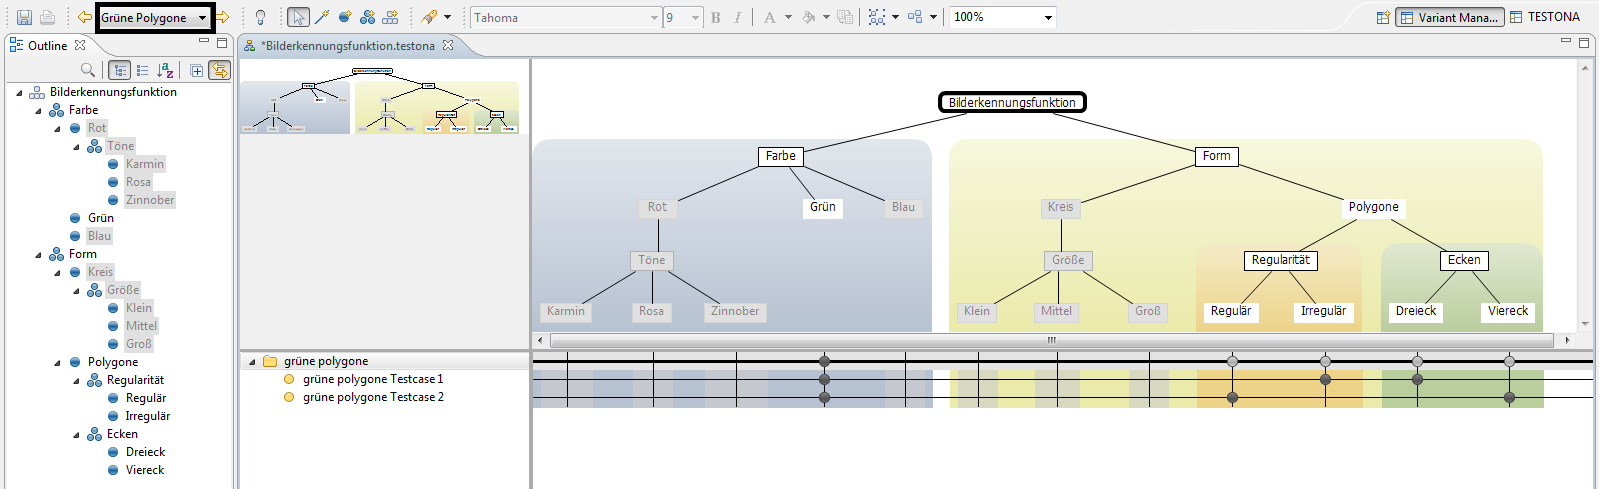
\includegraphics[scale=0.3]{gruenePolygone_DE.png}
  		  \caption{Richtige Auswahl der Klassen und Klassifikationen für die Testfallgenerierung}
     \label{ttn.gruen}
  \end{center}
\end{figure}


\begin{figure}[h]
  \begin{center}
    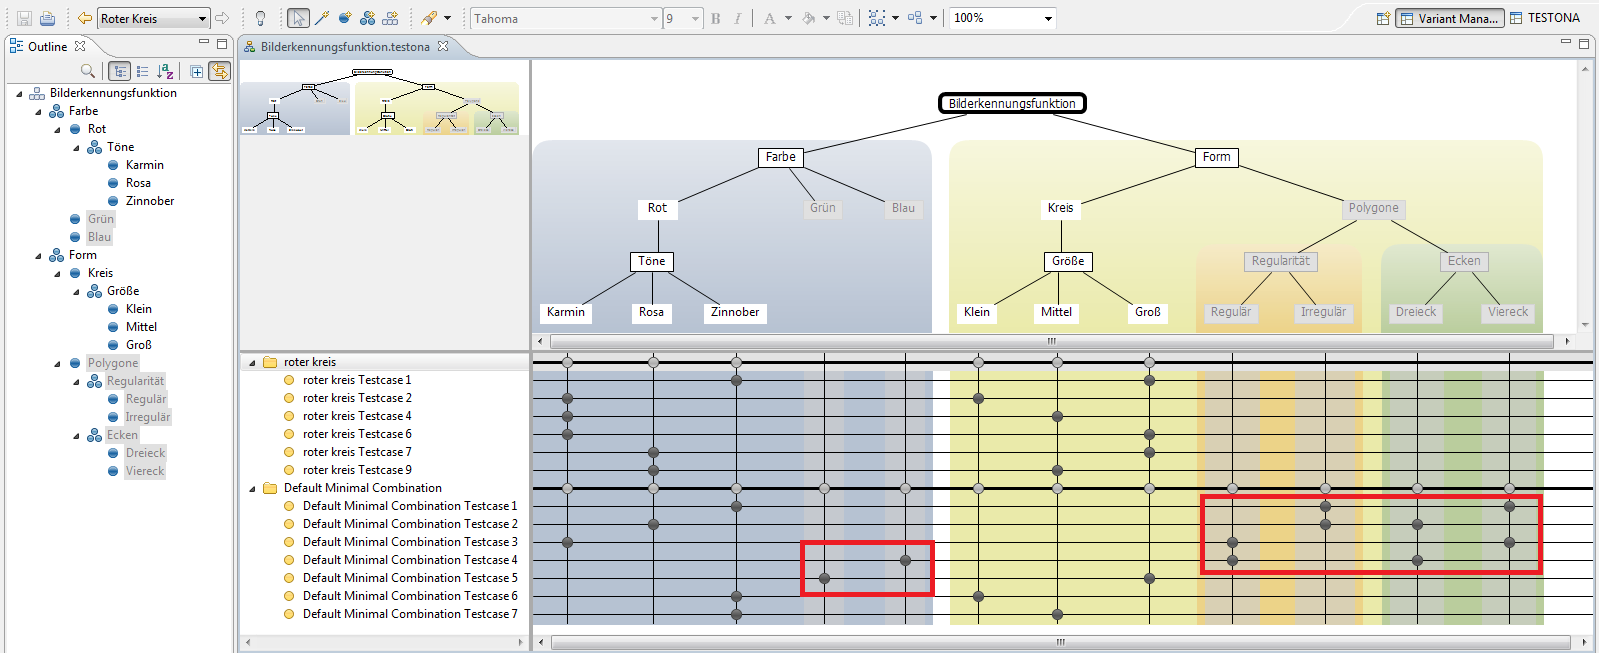
\includegraphics[scale=0.3]{roterKreis_DE.png}
  		  \caption{Ungültige Auswahl der Klassen (Grün und Blau) und Klassifikationen (Regularität und Ecken) für die Testfallgenerierung}
     \label{ttn.rot}
  \end{center}
\end{figure}


%#######################################################################################
%#######################################################################################
\newpage
\section{Variantenmanagement Software}
\paragraph{}
Die Erweiterung des schon vorhandenen Variantenmanagements in TESTONA wird dazu beitragen eine bessere Kopplung zwischen DOORS und TESTONA zu erzielen. Nach der Recherche über schon vorhandene Lösungen zu dieser Problemfrage bin ich auf keine brauchbare Implementation die in TESTONA angewendet werden kann gestoßen. Da es unter dem Begriff \glqq Variante\grqq~ viel Freiraum gibt, sind vorhandenen Lösungen sehr Problemspezifisch.\\


Im englischen Sprechraum werden die Begriffe \glqq feature modelling\grqq~ und \glqq domain engineering\grqq~ benutzt. Unter \glqq domain engineering\grqq~ ist die Wiederverwendung von Wissensgebieten für die Produktion einer neuen Software zu verstehen \cite{DomainEng}. Obwohl beide Begriffe sich auf die Softwareentwicklung spezialisieren, werden die Prinzipien allgemein in der Produktion verschiedener Produkte verwendet. Betrachtet man TESTONA, so sind die Editionen Light, Express, Professional und Enterprise Varianten.\\


Es existiert bereits Software die das Variantenmanagement unterstützt. Aber es gibt keine Software die eine Schnittstelle zu einer Datenbank zur Verfügung stellt. Weiterhin wird der Import von Varianten aus der Datenbank nicht begünstigt.\\


Die Firma \glqq Razorcat Development GmbH\grqq~ bietet auch einen Klassifikationsbaumeditor der TESTONA sehr ähnlich ist. Nach meiner Kenntnis hat diese Software keine Schnittstelle zu einer Datenbank und implementiert kein Variantenmanagement\footnote{http://www.razorcat.eu/cte.html, 15/11/2014}.



%#######################################################################################
%#######################################################################################
\newpage
\section{Neue Anforderungen}
\paragraph{}

Im Laufe des Projektes haben sich die Anforderungen leicht verändert. Die Parameterersetzung wird als Hauptpunkt dieser Arbeit betrachtet. Die in DOORS Module definierten Parameterwerte sollen in TESTONA importiert und angezeigt werden. Die Zuordnung von Parametern an Baumelemente erfolgt über die Verknüpfung von (aus DOORS importiert) Anforderungen mit einem Baumelement. In jeder dieser Varianten kann der Parameter einen anderen Wert darstellen. Bei Änderung der Variantenansicht in TESTONA soll der jeweilige Parameterwert für die aktive Variante angezeigt werden.\\


Die Abhängigkeitsregeln sollen das Variantenmanagement nicht mehr so sehr beeinflussen. Sie  sollen  enger mit der Testfallgenerierung verbunden sein als mit den einzelnen Varianten. Es wird davon ausgegangen, dass der Benutzer von TESTONA nur gültige Abhängigkeitsregeln deklariert hat.\\


Weiterhin sollen Optimierungsschritte bei der Testgenerierung betrachtet werden. Anhand der Parameterwerte kann es dazu kommen, dass doppelte Testfälle erstellt werden. Wenn die Endknoten unter einen Knoten die gleichen Werte besitzen, können vorher gültige Testfälle dadurch verdoppelt werden. Dabei soll der Benutzer auf die doppelten Testfälle aufmerksam gemacht werden oder diese Testfälle sollen automatisch gelöscht werden.